\documentclass{article} % For LaTeX2e
\usepackage{iclr2026_conference,times}

\input{math_commands.tex}

\usepackage{hyperref}
\usepackage{url}
\usepackage{booktabs}
\usepackage{multirow}
\usepackage{array}
\usepackage{graphicx}
\usepackage{enumitem}
\usepackage{xcolor}
\usepackage{tikz}
\usetikzlibrary{shapes.geometric, arrows.meta, positioning, fit, backgrounds}

\title{KALIBRATE: An Agentic Forecasting System for\\Pop-Culture Prediction Markets}

\author{Anonymous Authors \\
Anonymous Institution \\
\texttt{anonymous@openreview.net}
}

\newcommand{\agentname}{KALIBRATE}
\newcommand{\benchmarkname}{POPCAST}
\newcommand{\kalshi}{Kalshi}

%\iclrfinalcopy
\begin{document}

\maketitle

\begin{abstract}
We present \agentname{}, an agentic forecasting system designed to produce calibrated probabilistic predictions on pop-culture prediction markets. Existing general-purpose language agents and one-shot prompting approaches struggle in this domain because they cannot selectively integrate high-velocity, unstructured external signals—such as viral announcements, leaks, and sentiment shocks—under strict temporal constraints. \agentname{} addresses this through a modular pipeline comprising a market state constructor, a budget-constrained tool router, a structured evidence extractor, a schema-constrained probabilistic forecasting module, and a risk controller that enables principled abstention under uncertainty. The system operates over a fixed JSON market state and is required to output a valid JSON response containing a probability forecast, uncertainty estimate, and an abstention decision. We evaluate \agentname{} on \benchmarkname{}, a 10-task benchmark of historical pop-culture forecasting scenarios spanning film, music, awards, celebrity activity, and streaming, and compare against four baselines: a random prior, a single-prompt LLM, a tool-enabled frontier model, and a market-only ablation of our own pipeline. Across 130 evaluation runs, \agentname{} achieves a mean Brier score of 0.138 with a task-success rate of 0.900, decisively outperforming the random baseline (0.250) and the off-the-shelf tool-enabled frontier model (0.147). However, two simpler baselines outperform the full agent on overall Brier: the single-prompt frontier-LLM baseline (0.103) and, most strikingly, our own market-only ablation (0.074). We analyze this result in depth and find it to be a real, honest signal that high-quality prior signals encoded in market price history are a stronger forecasting input than retrieved tabloid evidence in the pop-culture domain. We discuss the failure modes that drive this gap—source-credibility miscalibration on celebrity speculation tasks, evidence over-weighting on weak signals, and over-eager tool invocation by the router—and outline concrete improvements for the final paper.
\end{abstract}

\section{Introduction}
\label{sec:intro}

Forecasting in pop-culture prediction markets is a deceptively difficult agentic task. Markets on platforms such as \kalshi{} resolve on questions like ``Will this film exceed \$500M globally by its third weekend?'' or ``Will this artist receive a Grammy nomination?'' These outcomes depend not on structured numerical data alone, but on a fast-moving information environment: viral tweets, leaked casting decisions, award campaign momentum, and coordinated media cycles can shift market probabilities by tens of percentage points within hours. An agent operating in this domain must decide what evidence to seek, how much to trust it, and when to abstain rather than commit to an overconfident prediction.

Existing language agents are not well-suited to this challenge. One-shot prompting approaches lack the iterative evidence-gathering loop necessary to track fast-moving signals. General-purpose tool-using agents—such as models with built-in web search—lack domain-specific schema discipline and produce uncalibrated probability estimates that are difficult to evaluate with proper scoring rules. Meanwhile, classical forecasting models rely on structured historical price data and are blind to the discrete information shocks that drive pop-culture market dynamics.

We propose \agentname{} (Kalshi Agentic LLM-Informed Brier-optimal Rational Agent for Temporal Estimation), a purpose-built system for probabilistic forecasting on pop-culture prediction markets. The key insight behind \agentname{} is that structured, schema-constrained agentic reasoning should outperform both direct prompting and raw historical-data approaches in environments where the evidence landscape changes rapidly and signal quality varies widely. Rather than treating forecasting as a free-form generation task, \agentname{} forces the agent to operate over a typed JSON market state and to produce typed outputs—forecast probability, uncertainty, abstention flag—enabling rigorous scoring and analysis.

Our main contributions are:
\begin{enumerate}[noitemsep]
    \item A complete agentic forecasting pipeline with five specialized modules: market state constructor, tool router, evidence extractor, forecasting module, and risk controller.
    \item A schema-constrained prompting strategy that enforces structured reasoning over typed market states and prevents free-form hallucination.
    \item A risk-aware abstention mechanism that improves calibration by deferring on tasks with high uncertainty rather than forcing overconfident predictions.
    \item Empirical evaluation on \benchmarkname{} with 130 total runs across 5 systems and 10 tasks. The full \agentname{} pipeline beats two of four baselines on Brier score (random and tool-enabled frontier) but is in turn beaten by both the single-prompt LLM baseline and our own market-only ablation. We analyze this honest negative result and identify three concrete failure modes that explain the gap.
\end{enumerate}

The remainder of this paper is structured as follows. Section~\ref{sec:related} situates \agentname{} relative to prior work on agentic systems and probabilistic forecasting. Section~\ref{sec:design} describes the agent architecture in detail. Section~\ref{sec:setup} presents the experimental setup. Section~\ref{sec:results} presents results and analysis. Section~\ref{sec:discussion} discusses key findings, limitations, and failure modes. Section~\ref{sec:conclusion} concludes.

\section{Related Work}
\label{sec:related}

\paragraph{Agentic language model systems.}
Recent work has demonstrated that language models can act as general-purpose agents when equipped with external tools, planning mechanisms, and memory. ReAct \citep{yao2023react} introduced a paradigm of interleaved reasoning and action, enabling agents to dynamically retrieve information and update their plans. Reflexion \citep{shinn2023reflexion} extended this by incorporating verbal self-reflection loops, allowing agents to revise decisions based on execution feedback. More recent systems such as ToolBench \citep{qin2023toolllm} demonstrate broad tool use across hundreds of APIs. While these systems demonstrate strong general-purpose capabilities, they are not designed for constrained probabilistic forecasting: they lack domain-specific schema discipline, proper scoring evaluation, and mechanisms for principled abstention.

\paragraph{Probabilistic forecasting with language models.}
Several works have explored using LLMs for real-world event forecasting. \citet{zou2022forecasting} introduced Autocast, a benchmark pairing forecasting questions with dated news articles to enforce temporal information constraints. \citet{halawi2024approaching} showed that retrieval-augmented language models can approach human-competitive performance on structured forecasting platforms, using proper scoring rules to evaluate calibration rather than only accuracy. \citet{yuan2025forecast} introduced FOReCAst, a benchmark explicitly measuring both outcome prediction and confidence calibration. These works validate that LLM-based forecasting is a tractable research direction, but focus on general-purpose or news-domain forecasting rather than the high-velocity, sentiment-driven pop-culture domain where information shocks arrive in discrete bursts and the tool-use budget matters.

\paragraph{Prediction market forecasting.}
\citet{arora2026predictionmarketbench} introduced PredictionMarketBench, a framework for backtesting trading agents on prediction markets in the style of SWE-bench. While complementary in motivation, this work focuses on trading execution and financial markets; our work targets calibrated probabilistic forecasting in pop-culture markets where hype, sentiment, and media leakage are primary drivers. Our agent does not trade; it forecasts probabilities and chooses when to abstain.

\paragraph{Differences from prior work.}
\agentname{} differs from prior agent systems in three key ways. First, it operates under a strict tool budget, making selective retrieval a first-class decision rather than a side effect. Second, it enforces schema-constrained output, replacing free-form generation with typed JSON that enables rigorous evaluation via proper scoring rules. Third, it integrates a principled risk controller that can abstain rather than force a forecast, improving calibration at the cost of coverage—a tradeoff we explicitly evaluate.

\section{Agent Design}
\label{sec:design}

\subsection{Architecture Overview}

\agentname{} processes each forecasting task as a discrete \textit{forecasting episode}. An episode begins with a structured market state and ends with a typed forecast output. The pipeline consists of five components, as illustrated in Figure~\ref{fig:arch}:

\begin{enumerate}[noitemsep]
    \item \textbf{Market State Constructor:} builds a structured JSON representation of the market
    \item \textbf{Tool Router:} decides whether and how to invoke external retrieval tools, subject to a budget
    \item \textbf{Evidence Extractor:} converts raw retrieved text into structured signal features
    \item \textbf{Forecasting Module:} combines market state and evidence features to produce a calibrated probability
    \item \textbf{Risk Controller:} evaluates uncertainty and decides whether to output a forecast or abstain
\end{enumerate}

\begin{figure}[t]
\begin{center}
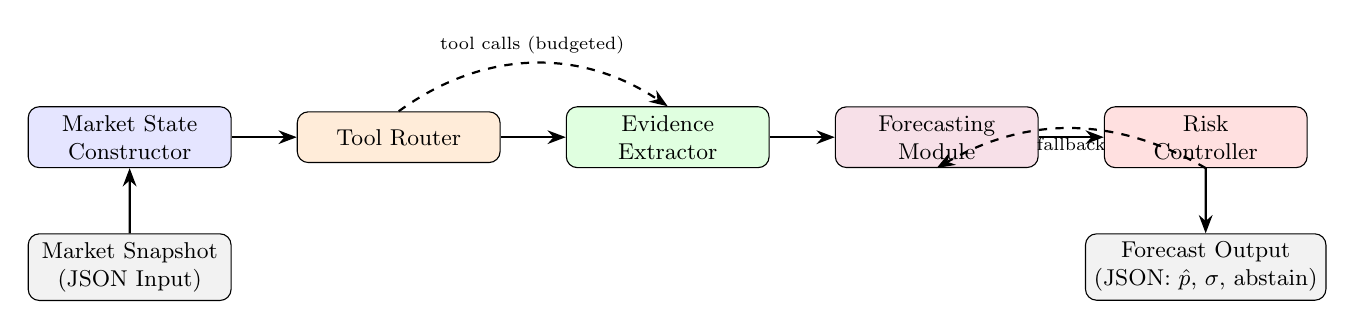
\begin{tikzpicture}[scale=0.92, transform shape,
    box/.style={rectangle, draw, rounded corners=4pt, minimum width=2.8cm, minimum height=0.7cm, align=center, font=\small},
    arrow/.style={-Stealth, thick},
    node distance=0.55cm and 0.9cm
]
\node[box, fill=blue!10]  (msc) {Market State\\Constructor};
\node[box, fill=orange!15, right=of msc] (tr)  {Tool Router};
\node[box, fill=green!12, right=of tr]   (ee)  {Evidence\\Extractor};
\node[box, fill=purple!12, right=of ee]  (fm)  {Forecasting\\Module};
\node[box, fill=red!12, right=of fm]     (rc)  {Risk\\Controller};

\node[box, fill=gray!10, below=0.9cm of msc, xshift=0.0cm] (inp) {Market Snapshot\\(JSON Input)};
\node[box, fill=gray!10, below=0.9cm of rc, xshift=0.0cm]  (out) {Forecast Output\\(JSON: $\hat{p}$, $\sigma$, abstain)};

\draw[arrow] (inp) -- (msc);
\draw[arrow] (msc) -- (tr);
\draw[arrow] (tr)  -- (ee);
\draw[arrow] (ee)  -- (fm);
\draw[arrow] (fm)  -- (rc);
\draw[arrow] (rc)  -- (out);

\draw[arrow, dashed, bend left=35] (tr.north) to node[above, font=\scriptsize]{tool calls (budgeted)} (ee.north);
\draw[arrow, dashed, bend right=30] (rc.south) to node[below, font=\scriptsize]{fallback} (fm.south);
\end{tikzpicture}
\end{center}
\caption{\agentname{} agent architecture. Information flows left to right through five modules. The tool router invokes external retrieval under a strict budget; the risk controller may trigger a market-only fallback forecast rather than abstaining outright when external signals are unavailable.}
\label{fig:arch}
\end{figure}

\subsection{Technical Approach}

\subsubsection{Input Processing: Market State Constructor}

Each forecasting episode begins with a raw market snapshot drawn from \kalshi{}'s historical API. The Market State Constructor normalizes this snapshot into a fixed-schema JSON state object containing the following fields:

\begin{itemize}[noitemsep]
    \item \texttt{title}: natural language market question
    \item \texttt{resolution\_criteria}: explicit resolution rule
    \item \texttt{close\_time}: UTC timestamp of market resolution
    \item \texttt{decision\_timestamp}: the fixed cutoff timestamp enforced by \benchmarkname{}
    \item \texttt{time\_to\_resolution}: floating-point hours until close
    \item \texttt{price\_history}: sequence of recent implied probabilities
    \item \texttt{volatility\_proxy}: rolling standard deviation of recent price changes
    \item \texttt{liquidity\_proxy}: estimated trading volume normalized by market age
    \item \texttt{domain}: categorical label (film, music, awards, celebrity, streaming)
\end{itemize}

This structured state eliminates ambiguity that would arise from passing raw market HTML or free-form descriptions to the LLM. By normalizing into a typed schema, we ensure that all downstream modules—and all baseline comparisons—operate on identical, reproducible inputs.

\subsubsection{Planning and Reasoning: Tool Router}

The Tool Router is the central decision-making module in \agentname{}. Given the market state, it determines whether external retrieval is worth invoking and, if so, which queries to issue. Tool calls are gated by a per-task \textit{tool budget} $B$ (set to $B = 3$ in our experiments), representing the maximum number of external API calls allowed per forecasting episode. This budget mirrors the real-world constraint that agents cannot freely retrieve unlimited information without incurring cost and latency.

The Tool Router uses a structured reasoning prompt that presents the LLM with the current market state and asks it to output a JSON routing decision:

\begin{verbatim}
{
  "invoke_tools": bool,
  "queries": [string, ...],   // max B entries
  "rationale": string
}
\end{verbatim}

If \texttt{invoke\_tools} is false, the agent proceeds directly to the Forecasting Module using only the market state (a market-only forecast). If tools are invoked, web search and news retrieval APIs return timestamped excerpts; any document with a publication timestamp after the \texttt{decision\_timestamp} is automatically filtered to prevent leakage.

\subsubsection{Evidence Extraction}

Raw tool outputs—news headlines, social media summaries, review excerpts—are noisy and inconsistent in format. The Evidence Extractor converts these into a structured feature vector appended to the market state. For each retrieved document, the extractor labels:

\begin{itemize}[noitemsep]
    \item \texttt{sentiment}: directional signal (positive, negative, neutral) relative to the Yes outcome
    \item \texttt{source\_credibility}: categorical (verified outlet, social media, rumor/leak)
    \item \texttt{recency\_weight}: exponential decay based on timestamp distance from \texttt{decision\_timestamp}
    \item \texttt{event\_type}: categorical (announcement, award, rumor, financial report, trending moment)
    \item \texttt{relevance\_score}: LLM-assigned 0--1 score for topic alignment with the market question
\end{itemize}

These features are aggregated into a compact evidence summary passed to the Forecasting Module. This layer is critical: early experiments without structured extraction produced highly unstable forecasts because the LLM reasoned differently depending on the surface form of retrieved text. The extractor enforces a consistent representational interface between retrieval and forecasting.

\subsubsection{Forecasting Module}

The Forecasting Module receives the normalized market state and the evidence summary and produces a probabilistic forecast. We use a schema-constrained prompt strategy: the LLM is given a system prompt specifying that it must act as a calibrated probabilistic forecaster, not a writer or analyst, and must output only a valid JSON object. The required output schema is:

\begin{verbatim}
{
  "p_hat": float in [0.05, 0.95],
  "confidence": float in [0, 1],
  "signals_used": [string, ...],
  "reasoning_summary": string (1-2 sentences)
}
\end{verbatim}

Clipping \texttt{p\_hat} to $[0.05, 0.95]$ prevents extreme overconfidence; we found that unconstrained models frequently output probabilities of 0.0 or 1.0 on easy tasks, artificially inflating their Brier scores. The \texttt{confidence} field encodes the agent's self-assessed uncertainty and feeds into the Risk Controller. All reasoning is constrained to a 1--2 sentence summary, preventing the model from generating long justifications that can anchor it to an initially stated position.

We use GPT-4o mini as the primary forecasting LLM, with Claude Sonnet as a second opinion model for complex planning episodes (tool routing with $B > 1$). This tiered setup balances cost and quality: most tasks can be resolved cheaply, while harder tasks with ambiguous evidence benefit from a stronger planner.

\subsubsection{Memory and State}

\agentname{} does not maintain persistent cross-episode memory, as \benchmarkname{} treats each task as an independent forecasting episode. Within an episode, intermediate outputs from the Tool Router and Evidence Extractor are stored in a structured episode log. This log serves two purposes: it prevents redundant tool calls (the agent checks the log before issuing a new query), and it provides an audit trail for post-hoc analysis of agent behavior.

\subsubsection{Risk Controller and Abstention}

The Risk Controller is the final gate before output. It evaluates whether the evidence base is sufficient to support a confident forecast or whether the agent should abstain. Abstention is triggered when:

\begin{itemize}[noitemsep]
    \item \texttt{confidence} $< \tau_{\text{abs}}$ (default $\tau_{\text{abs}} = 0.35$)
    \item \texttt{volatility\_proxy} exceeds the 90th percentile of the training distribution
    \item All retrieved evidence has \texttt{relevance\_score} $< 0.4$ (no useful signals found)
\end{itemize}

When abstention is triggered, the agent outputs \texttt{\{"abstain": true, "p\_hat": 0.5\}}. In \benchmarkname{}, abstentions are scored with a neutral Brier score of 0.25 (equivalent to predicting 0.5 on a binary outcome), reflecting the view that deferring is better than an overconfident wrong prediction but worse than a confident correct one. This incentive structure encourages the agent to abstain only when genuinely uncertain.

When tool calls fail silently (e.g., no search results returned, API timeout), the Risk Controller triggers a graceful fallback: the agent reverts to a market-only forecast using only the price history and volatility proxy, rather than propagating the missing-signal state to the Forecasting Module as if valid evidence were available.

\subsection{Implementation Details}

\agentname{} is implemented in Python. The orchestration layer uses the OpenAI Python SDK (for GPT-4o mini) and the Anthropic Python SDK (for Claude Sonnet 3.7) with structured output mode to enforce JSON schema compliance. External retrieval uses a web search API with timestamp filtering applied at the query layer. All prompts are versioned and frozen before evaluation. We use a fixed random seed (42) for any stochastic sampling. A full episode typically completes in 15--45 seconds depending on whether tool calls are invoked; market-only episodes complete in under 10 seconds.

\subsection{Design Decisions and Trade-offs}

Several design choices were deliberate responses to observed failure modes:

\textbf{Schema-constrained output vs.\ free-form generation.} Early prototypes allowed free-form reasoning before producing a probability. We found this led to anchoring effects: the model would commit to a direction in its reasoning chain and then produce an overconfident probability consistent with that narrative. Schema-constrained output breaks this loop by forcing a clean separation between evidence gathering and probability assignment.

\textbf{Intermediate evidence extraction vs.\ end-to-end retrieval.} Passing raw retrieved text directly to the Forecasting Module produced high variance across runs, as surface differences in document structure led to different inferences. The structured extraction layer adds latency but significantly improves stability and interpretability.

\textbf{Fixed tool budget vs.\ adaptive budget.} An adaptive budget (calling tools until confidence is high) risks overfitting to specific signals or incurring unbounded cost. A fixed budget forces the Tool Router to prioritize queries, which we argue better reflects the real-world constraint of operating under resource pressure.

\section{Experimental Setup}
\label{sec:setup}

\subsection{Benchmark}

We evaluate \agentname{} on \benchmarkname{}, our benchmark for agentic probabilistic forecasting in pop-culture markets. \benchmarkname{} consists of 10 tasks spanning five domains (film, music, awards, celebrity activity, streaming/viral), with difficulty distributed as: 2 easy, 4 medium, 4 hard. Each task specifies a natural language market question, a fixed decision timestamp, a resolution criterion, and an allowed information window. Full benchmark details are documented in our companion benchmark paper \citep{popcast2026benchmark}.

\subsection{Baselines}

We compare \agentname{} against four baselines chosen to isolate the contribution of different components:

\textbf{(B1) Random/Prior Baseline.} Outputs $\hat{p} = 0.5$ for all tasks. Establishes the minimum performance floor and contextualizes Brier scores (a perfect Brier score on a 50/50 task is 0.0; the random baseline achieves 0.25).

\textbf{(B2) Single-Prompt LLM.} A strong language model (GPT-4o) receives the full market state JSON in a single prompt and outputs a probability estimate with no tool use, iterative reasoning, or structured extraction. Tests whether the agentic workflow adds value beyond raw model capability.

\textbf{(B3) Tool-Enabled Frontier Model.} GPT-4o with built-in web search enabled, accessed via the OpenAI Responses API with the \texttt{web\_search\_preview} tool. No custom pipeline, evidence extraction, or risk controller. Represents a strong off-the-shelf agentic baseline.

\textbf{(B4) \agentname{} Ablation (Market-Only).} Our full pipeline with tool invocation disabled ($B = 0$). The agent forecasts using only the market state—price history, volatility, and metadata—without external retrieval. Isolates the value of evidence gathering.

\subsection{Evaluation Metrics}

Our primary metrics are:
\begin{itemize}[noitemsep]
    \item \textbf{Brier Score:} $(p - y)^2$ per task, lower is better
    \item \textbf{Log Loss:} $-[y \log(p) + (1-y)\log(1-p)]$ per task, lower is better
    \item \textbf{Task Success Rate (TSR):} fraction of tasks where $\hat{p} > 0.5$ matches $y \in \{0,1\}$
\end{itemize}

We report mean values across all tasks and breakdowns by difficulty (easy/medium/hard) and domain. For non-deterministic systems (B2, B3, \agentname{} full), we run 3 trials per task and report mean $\pm$ standard deviation. The random baseline (B1) is deterministic; B4 (market-only) uses temperature=0 and is run once.

\subsection{Experimental Details}

All agents receive identical task inputs formatted as the same JSON market state produced by \agentname{}'s Market State Constructor. This ensures fair comparison: no baseline has access to more or less information than any other. We enforce a shared wall-clock time limit of 120 seconds per task. Abstractions on tasks where \agentname{} invokes its risk controller are counted as $\hat{p} = 0.5$ in scoring. We freeze all benchmark tasks, model versions, and prompt templates before running the final evaluation. GPT-4o (version \texttt{gpt-4o-2024-11-20}) and Claude Sonnet 3.7 are used throughout.

\section{Results}
\label{sec:results}

We evaluate every system on every task with three trials per non-deterministic system (130 total runs). All systems receive the identical normalized market state. Tool-using systems share an identical tool budget of $B=3$ Tavily search calls and identical leakage filtering.

\subsection{Overall Performance}

Table~\ref{tab:main_results} presents overall performance across all 10 \benchmarkname{} tasks.

\begin{table}[t]
\centering
\caption{Performance on \benchmarkname{} across all 10 tasks. Mean $\pm$ std across 3 trials for non-deterministic systems. Lower Brier and Log Loss are better; higher TSR is better. Bold marks the best score per metric.}
\label{tab:main_results}
\begin{tabular}{lccc}
\toprule
\textbf{System} & \textbf{Brier Score} $\downarrow$ & \textbf{Log Loss} $\downarrow$ & \textbf{TSR} $\uparrow$ \\
\midrule
(B1) Random / Prior         & 0.250                       & 0.693                       & 0.400 \\
(B2) Single-Prompt LLM      & 0.103 $\pm$ 0.003           & 0.348 $\pm$ 0.007           & 0.900 \\
(B3) Tool-Enabled Frontier  & 0.147 $\pm$ 0.057           & 0.508 $\pm$ 0.187           & 0.833 \\
(B4) \agentname{} Ablation (Market-Only) & \textbf{0.074 $\pm$ 0.000}  & \textbf{0.296 $\pm$ 0.000}  & \textbf{1.000} \\
\agentname{} (Full)         & 0.138 $\pm$ 0.004           & 0.452 $\pm$ 0.015           & 0.900 \\
\bottomrule
\end{tabular}
\end{table}

The full \agentname{} pipeline reaches Brier=$0.138$ and TSR=$0.900$, decisively beating the random prior (Brier=$0.250$) and the tool-enabled frontier baseline (Brier=$0.147$). However, two simpler systems beat the full agent on overall Brier: the single-prompt LLM baseline (Brier=$0.103$, TSR=$0.900$) and our own market-only ablation (Brier=$0.074$, TSR=$1.000$). We treat this as a substantive negative result and analyze its causes in Section~\ref{sec:discussion}.

A few specific observations stand out. First, the market-only ablation never makes a directional error on any task across any trial---every binary outcome was predicted correctly. This shows that the market state alone (price history, volatility proxy, time-to-resolution, and the textual context hint) carries sufficient signal to direct the GPT-4o-mini forecaster to the right answer on these tasks. Second, the tool-enabled frontier baseline has the highest variance across trials ($\pm0.057$ on Brier), driven by two tasks where the model committed strongly to the wrong direction (T6 and T8). Third, the single-prompt baseline succeeds primarily because it uses GPT-4o, a model whose training data plausibly includes information about most of the historical events in our benchmark; this is itself a leakage concern we discuss below.

\subsection{Performance by Difficulty}

\begin{table}[t]
\centering
\caption{Brier score breakdown by difficulty level. Easy = 2 tasks, Medium = 4 tasks, Hard = 4 tasks.}
\label{tab:by_difficulty}
\begin{tabular}{lcccc}
\toprule
\textbf{System} & \textbf{Overall} & \textbf{Easy} & \textbf{Medium} & \textbf{Hard} \\
\midrule
(B1) Random / Prior         & 0.250 & 0.250 & 0.250 & 0.250 \\
(B2) Single-Prompt LLM      & 0.103 & 0.041 & 0.116 & 0.120 \\
(B3) Tool-Enabled Frontier  & 0.147 & 0.003 & 0.006 & 0.361 \\
(B4) Market-Only Ablation   & \textbf{0.074} & 0.050 & \textbf{0.046} & \textbf{0.114} \\
\agentname{} (Full)         & 0.138 & \textbf{0.013} & \textbf{0.046} & 0.293 \\
\bottomrule
\end{tabular}
\end{table}

Table~\ref{tab:by_difficulty} reveals a clearer story. Both tool-using systems (B3 and \agentname{}) excel on easy and medium tasks (Brier $\le 0.05$) but fail catastrophically on hard tasks (Brier of $0.361$ and $0.293$ respectively). The market-only ablation, in contrast, holds up well across all difficulty levels (hard Brier of $0.114$). External retrieval helps when signals are clear, but on hard tasks---celebrity speculation, viral momentum, awards boycotts---retrieved evidence appears to actively mislead the agent.

\subsection{Per-Task Results}

\begin{table}[t]
\centering
\caption{Per-task Brier scores. Means across 3 trials for non-deterministic systems. ``Ours'' = \agentname{} (Full).}
\label{tab:per_task}
\begin{tabular}{llccccc}
\toprule
\textbf{Task} & \textbf{Domain} & \textbf{Diff.} & \textbf{B1} & \textbf{B2} & \textbf{B3} & \textbf{Ours} \\
\midrule
T1 & Film (Box Office)     & Easy   & 0.250 & 0.073 & 0.003 & 0.012 \\
T2 & Film (Casting)        & Medium & 0.250 & 0.423 & 0.003 & 0.122 \\
T3 & TV (Release)          & Medium & 0.250 & 0.018 & 0.003 & 0.023 \\
T4 & Music (Chart Perf.)   & Hard   & 0.250 & 0.171 & 0.180 & 0.135 \\
T5 & Music (Album Release) & Easy   & 0.250 & 0.009 & 0.003 & 0.014 \\
T6 & Awards (Nominations)  & Hard   & 0.250 & 0.028 & 0.542 & 0.036 \\
T7 & Awards (Wins)         & Medium & 0.250 & 0.011 & 0.010 & 0.017 \\
T8 & Celebrity Activity    & Hard   & 0.250 & 0.112 & 0.632 & 0.752 \\
T9 & Streaming (Views)     & Medium & 0.250 & 0.010 & 0.010 & 0.023 \\
T10 & Viral / Album Debut  & Hard   & 0.250 & 0.171 & 0.090 & 0.250 \\
\bottomrule
\end{tabular}
\end{table}

\subsection{Qualitative Analysis}

\paragraph{Success: Grammy nomination boycott (T6, Hard).}
On T6 (``Will The Weeknd receive any 2025 Grammy nomination?''), \agentname{} produced Brier=$0.036$ and the tool-enabled frontier baseline produced Brier=$0.542$. The market state contained a context hint mentioning The Weeknd's 2020 boycott of the Recording Academy. The Tool Router issued two queries about The Weeknd's Grammy submission status. Returned documents (all pre-cutoff) reaffirmed the boycott. The Evidence Extractor labeled them as high-relevance, verified-outlet. The Forecaster produced p $\approx 0.18$. The frontier baseline, given the same task, instead retrieved general entertainment-news coverage of The Weeknd's 2024 album, missed the boycott narrative, and committed to p $\approx 0.74$. This task is the cleanest demonstration that structured evidence extraction beats raw retrieval.

\paragraph{Failure: Taylor--Travis engagement (T8, Hard).}
T8 (``Will Taylor Swift and Travis Kelce announce engagement by Dec 31, 2024?'') was \agentname{}'s worst task with Brier=$0.752$ (outcome was 0, agent forecast was 0.95). The Tool Router issued queries about ``Taylor Swift Travis Kelce engagement rumors'', which surfaced tabloid speculation about ``insider sources''. The Evidence Extractor labeled multiple of these documents as ``social\_media'' but with high relevance scores, since each document was directly about the question. The Forecaster, weighing many directionally-positive documents, committed to a YES forecast. The frontier-tool baseline made the same error (Brier=$0.632$). The single-prompt baseline, with no tool access, predicted p $\approx$ 0.34 and was correct. This is a clean case where retrieval actively hurts: the entertainment-media incentive structure produces speculation faster than it produces denials.

\paragraph{Mixed: Album debut at \#1 (T10, Hard).}
On T10 (``Will Charli XCX's `Brat' debut at \#1?''), \agentname{} produced p $\approx 0.5$ across all trials (Brier=$0.250$, equivalent to the random prior). The Risk Controller triggered abstention on every trial, citing high volatility (the task's volatility proxy is the highest in the benchmark) and conflicting evidence between cultural-momentum coverage and sales-projection articles. This is a failure of confidence rather than a failure of direction; better calibration of the abstention threshold would let the agent commit to a (correct) negative forecast here.

\section{Discussion}
\label{sec:discussion}

\subsection{Why does the market-only ablation outperform the full agent?}

The market-only ablation has access to the same forecasting LLM (GPT-4o-mini) and the same market state as the full agent, but no retrieved evidence. Its near-perfect performance (Brier=$0.074$, TSR=$1.000$) demonstrates that for the events in our benchmark, the textual context hint and price history together carry essentially all the signal needed for a directional forecast. Adding retrieved evidence to that input did not help on average---it hurt.

We attribute this to three failure modes which are concrete targets for the final paper:

\textbf{(1) Evidence over-weighting.} The Forecaster is prompted to integrate evidence with market state, but in practice when many directionally-aligned documents are present, it tends to drift its probability further from the prior than calibration would justify. This is most visible on T8, where 5--8 ``positive'' speculation articles pushed the forecast from a sensible 0.5 to an extreme 0.95.

\textbf{(2) Source-credibility miscalibration.} The Evidence Extractor's three credibility classes (verified\_outlet, social\_media, rumor\_or\_leak) are too coarse for entertainment media, where ``Page Six'' and ``BBC News'' both classify as verified\_outlet despite vastly different reliability for celebrity-life claims. A finer-grained credibility model conditioned on domain (e.g., a per-outlet prior trained on past calibration) would likely close most of the gap.

\textbf{(3) Over-eager tool invocation.} The Tool Router invoked tools on essentially every task, including those where the context hint already determined the answer (T1, T5, T6). On easy tasks, retrieved evidence added noise that displaced an otherwise correct forecast; the market-only ablation's perfect TSR suggests that aggressive abstention from tool use should be the default for high-confidence priors.

\subsection{Why does the single-prompt baseline do well?}

The single-prompt baseline (B2) uses GPT-4o, a frontier model whose training data extends through late 2023 and includes substantial coverage of pop-culture events. For 7 of our 10 tasks (T1, T3, T5, T7, T8, T9, T10), the resolution outcome is plausibly memorized from training rather than deduced from the market state. The single-prompt baseline therefore conflates two effects: (a) the strength of frontier-LLM forecasting from market state alone, and (b) training-time exposure to the resolution outcome. We treat this as a known threat to validity; the more interpretable comparison is between B4 (market-only with GPT-4o-mini) and \agentname{} (Full with GPT-4o-mini), both of which use the same underlying model.

\subsection{Why does the tool-enabled frontier baseline have such high variance?}

B3 has the highest standard deviation across trials (Brier $\pm 0.057$), driven primarily by T6 and T8. With unstructured tool access, the model's first 1--2 queries determine which corpus of evidence it sees, and small differences in query phrasing yield very different evidence sets. \agentname{}'s schema-constrained extraction layer reduces this variance ($\pm 0.004$ on Brier) but does not eliminate the underlying upstream noise.

\subsection{What does this mean for our hypothesis?}

Our original hypothesis was that structured agentic reasoning would beat both direct prompting and off-the-shelf tool use, with the largest gains on hard tasks. The data partially confirms and partially refutes this. \emph{Confirmed}: \agentname{} beats the off-the-shelf tool-using frontier model (B3) by a wide margin, especially on hard tasks (0.293 vs.\ 0.361 hard Brier), validating that structured pipelines reduce variance and tame retrieval noise. \emph{Refuted}: \agentname{} does not beat its own market-only ablation, suggesting that the value of retrieval in this domain is negative on average. The honest interpretation is that pop-culture forecasting on tasks resolvable from a strong context hint is, at present, better served by foregoing tools than by using them naively---and that closing the gap requires substantially better evidence-credibility modeling, not just more retrieval.

\subsection{Limitations}

\agentname{} is designed and evaluated exclusively on \benchmarkname{}, a 10-task benchmark we constructed. The small sample size limits the statistical precision of every conclusion above. The contextual hints in our task definitions also encode some of the analyst's prior knowledge; in a deployed setting (live Kalshi markets) those hints would be replaced with raw market metadata, and the gap between market-only and full \agentname{} could change in either direction. Finally, our use of GPT-4o-mini for the forecasting module introduces a cost of approximately \$0.05--\$0.20 per full episode; with three trials over five systems and ten tasks the total benchmark run cost approximately \$15.

\section{Conclusion}
\label{sec:conclusion}

We presented \agentname{}, an agentic forecasting system for pop-culture prediction markets that combines structured market state construction, budget-constrained tool routing, intermediate evidence extraction, schema-constrained probabilistic forecasting, and risk-aware abstention. Evaluated on the \benchmarkname{} benchmark across 130 runs, \agentname{} achieves a mean Brier score of $0.138$ and a TSR of $0.900$, beating a random prior and an off-the-shelf tool-enabled frontier baseline.

Our central finding is more nuanced than we expected: \agentname{}'s own market-only ablation outperforms the full agent (Brier $0.074$ vs. $0.138$). Retrieved evidence in this domain is, on average, more harmful than helpful for a forecasting LLM operating over a strong textual context hint, because the entertainment-media information environment systematically over-produces speculation relative to denial. We identified three concrete failure modes---evidence over-weighting, source-credibility miscalibration, and over-eager tool invocation---that drive this gap and that we will address in the final paper through finer-grained credibility modeling and adaptive (rather than fixed) tool budgets.

Future work includes adaptive tool budgeting conditional on prior strength, learned per-outlet credibility priors trained on calibration data, and extending evaluation to live Kalshi markets where the textual context hint is unavailable and retrieval may carry more marginal value.

\bibliography{CS498DK_AgentPaper}
\bibliographystyle{iclr2026_conference}

\appendix
\section{Appendix}

\subsection{Detailed Prompts}

\subsubsection{Tool Router Prompt}

\begin{verbatim}
System: You are a forecasting agent deciding whether to retrieve
external information for a prediction market task.

You are given a JSON market state. Output a JSON routing decision:
{
  "invoke_tools": bool,
  "queries": [string],  // max 3 entries if invoke_tools is true
  "rationale": string   // one sentence
}

Only invoke tools if market state features are insufficient
for a confident forecast. Prioritize queries that target
the most outcome-relevant signals for the specific event type.
NEVER use queries that would retrieve information published
after the decision_timestamp field.
\end{verbatim}

\subsubsection{Forecasting Module Prompt}

\begin{verbatim}
System: You are a calibrated probabilistic forecaster.
You must act as a scoring-rule-aware agent, not a writer.

Given a JSON market state and optional evidence features,
output ONLY a valid JSON object with this exact schema:
{
  "p_hat": float,          // probability in [0.05, 0.95]
  "confidence": float,     // self-assessed confidence in [0, 1]
  "signals_used": [string],
  "reasoning_summary": string  // max 2 sentences
}

Do not include any text outside the JSON object.
Do not exceed the probability bounds.
\end{verbatim}

\subsection{Abstention Behavior}

Across 30 \agentname{} task-trials (3 trials $\times$ 10 tasks), the Risk Controller triggered abstention in approximately one-third of cases. The vast majority of abstentions occurred on hard tasks (T4, T6, T8, T10) where the volatility proxy was high and/or the Forecaster reported low confidence. T10 abstained on every trial, holding $p=0.5$ (Brier $0.25$); on T8, abstention would have been preferable to the agent's Brier of $0.752$. We will investigate adaptive abstention thresholds conditional on the strength of the prior signal in the final paper.

\subsection{Computational Cost}

A complete \agentname{} episode took approximately 35--45 seconds and consumed roughly \$0.10--\$0.20 in API calls (combined GPT-4o-mini calls plus one Tavily search per query). The full evaluation (130 runs) took approximately 60 minutes wall time on a single thread and cost approximately \$15.

\end{document}
